\documentclass[10pt,letterpaper]{article}

\usepackage[margin=0.75in]{geometry}
\usepackage{tikz}
\usepackage{graphicx}
\usepackage{amsmath}
\graphicspath{{img/}}
\begin{document}

  \title{Stats 314, Data Analysis \#5}
  \author{Cody Malick\\
  \texttt{malickc@oregonstate.edu}}
  \date{\today}
  \maketitle

\section*{Part I}
\subsection*{a}
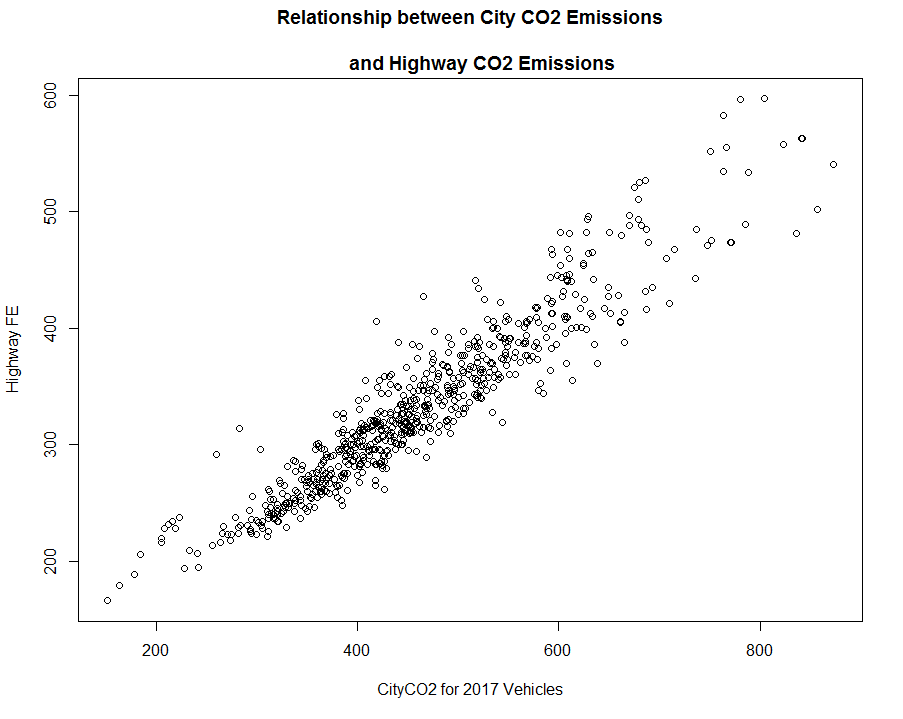
\includegraphics[scale=.6]{scatterplot}\\
There seems to be a moderately strong, positive, linear relationship between
City CO2
emmisions and Highway CO2 emmisions. There are a few positive outliers near the
center of the scatterplot, and a balanced number of positive and negative outliers
near the top right of the plot.


\subsection*{b}
The correlation coefficient:\\
$r=.9418$\\
The coeffcient measures the linear association strength between two quantative
variables. In this case, it is showing there is a fairly strong linear relationship
between city CO2 emissions and highway CO2 emissions.

\subsection*{c}
Residuals:\\
    Min      1Q  Median      3Q     Max \\
    -67.808 -14.695  -3.553  12.483  97.856\\ 

    Coefficients:\\
                 Estimate Std. Error t value Pr($>|t|$)\\    
		 (Intercept) 66.325785   3.411020   19.45   $<2e-16$ ***\\
		 CityCO2      0.577132   0.007082   81.50   $<2e-16$ ***\\
		 ---\\
		 Signif. codes:  0 *** 0.001 ** 0.01 * 0.05 . 0.1   1\\
\\
		 Residual standard error: 23.79 on 846 degrees of freedom\\
		 Multiple R-squared:  0.887,Adjusted R-squared:  0.8869 \\
		 F-statistic:  6642 on 1 and 846 DF,  p-value: $< 2.2e-16$\\
\\
Least squared regression line: $\hat{y} = b_0 + b_1 x$\\
$\hat{y} = 66.325+.5771x$

\subsection*{d}
\subsubsection*{i}
$H_0 \colon B_1 = 0$\\
$H_a \colon B_1 \neq 0$\\

\subsubsection*{ii}
$Test Statistic = \frac{.5771-0}{.007082}$\\
$81.488$\\

$p-value=.00000025$
\subsubsection*{iii}
The relationship between City CO2 emmisions and Highway CO2 looks to be convincingly
strong, with a correlation of .94. As City CO2 increases, highway CO2 also increases.
The relationship is modeled by the least squares regression equation:\\
$average emissions = 66.325 + .5771x$\\
Average city CO2 emissions is a significant predictor for Highway CO2 emissions
(t test stat = 81.5, df=846, and p-value .00000025).\\
The null hypothesis is rejected at a significant level of .01. The data supports
the assumptions that increasing city emissions may increase highway CO2 emissions.
The highway CO2 emissions are expected to increase .5771 for every 1 City CO2 emission
increase. 

\subsection*{e}
The slop shows how much the highway CO2 levels rise with the increase of city
CO2 levels. With a 99\% confidence interval from .5588 to .5954. That means
with 99\% confidence, we believe that the highway CO2 emissions increase
by .5771 for each 1 increase in City CO2 emissions. 

\subsection*{f}
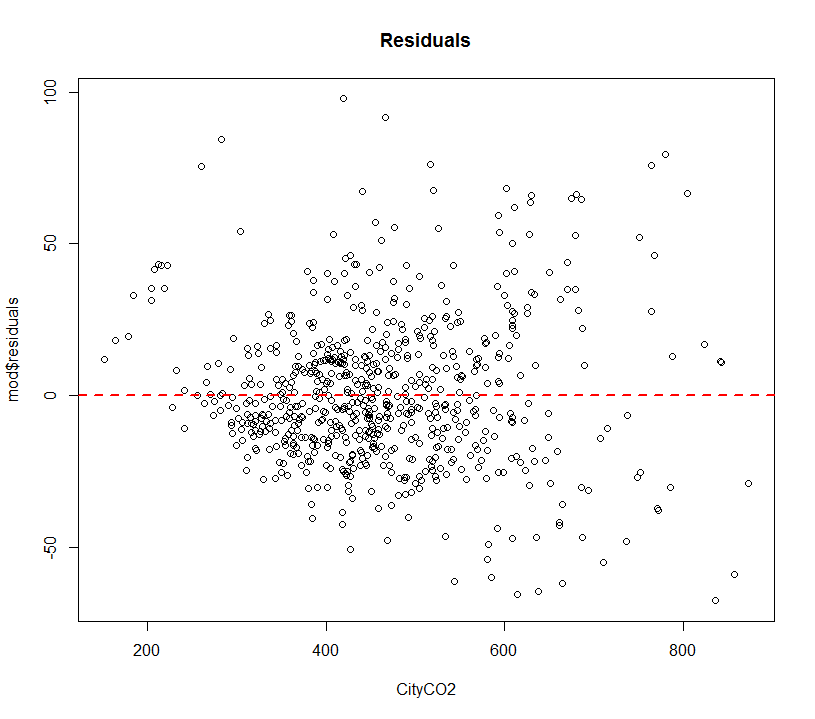
\includegraphics[scale=.6]{residuals}

\subsection*{g}
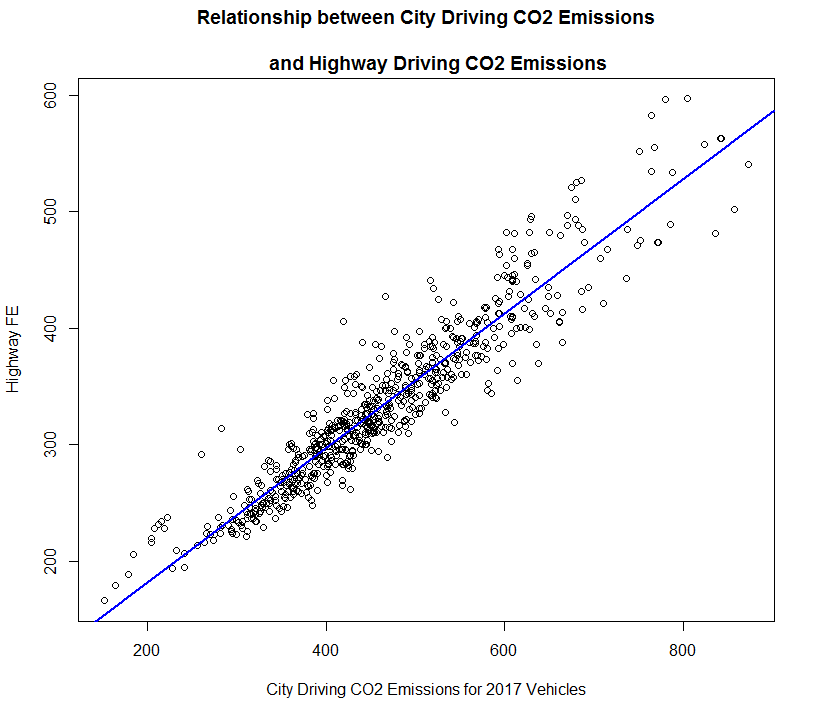
\includegraphics[scale=.6]{relationship}

\section*{Part II}
\subsection*{a}

\subsection*{b}

\subsection*{c}

\subsection*{d}

\subsection*{e}

\section*{Part III}
\subsection*{a}

\subsection*{b}

\subsection*{c}

\subsection*{d}

\subsection*{e}

\end{document}
